
The 1D geometry is based on geometrical parameters of a single strand of a skew quadrupole whose simulations are further described in chapter \ref{section:skew_quadrupole_quench_detection_analysis}. As presented in Fig. \ref{fig: 1d_strand_geometry}, it consists of a 1 m-long strand with a circular cross-section (in yellow). It is made of Nb-Ti with copper as a stabiliser. The strand is fully insulated with an S2-glass material (in red). Then, it is immersed in D10 epoxy resin (in blue) \cite{hl_lhc_tech_design_report_v01}.

\begin{figure}[H]
    \centering
    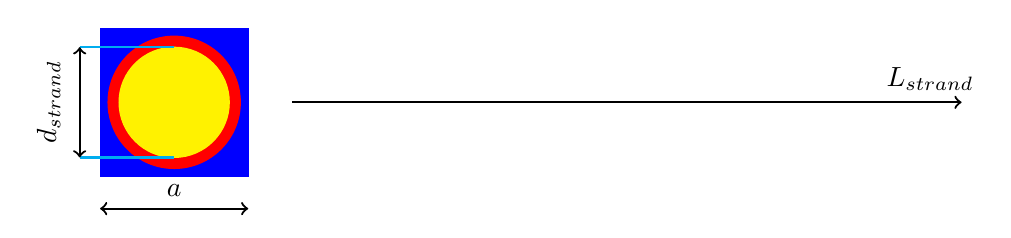
\begin{tikzpicture}[scale = 1]
        \filldraw[blue] (-0.941,-0.941) rectangle (0.941,0.941);
        \filldraw[red] (0,0) circle (0.7+0.07*2);
        \filldraw[yellow] (0,0) circle (0.7);
        \draw[thick, cyan] (-0.8*1.5,0.7) -- (0,0.7);
        \draw[thick, cyan] (-0.8*1.5,-0.7) -- (0,-0.7);
        \draw[black, thick, <->] (-0.75*1.6,0.7) -- (-0.75*1.6,-0.7);
        \node[scale = 1, rotate=90] at (-1.1*1.45, 0) {$d_\text{strand}$};
        \draw[thick,<->] (-0.941,-0.9*1.5) -- (0.941,-0.9*1.5);
        \node[scale = 1] at (0, -0.7*1.6) {$a$};
        \draw[thick,->] (1.5,0) -- (10.0,0);
        \node[scale = 1] at (9.6, 0.3) {$L_\text{strand}$};
    \end{tikzpicture}
    \caption{1D strand geometry}
    \label{fig: 1d_strand_geometry}
\end{figure}

\begin{table}[h!]
    \caption{Geometrical strand parameters} 
    \vspace{-1.em} 
    \fontsize{10}{10}
    \selectfont 
    \renewcommand{\arraystretch}{1.5}
    \begin{center}
        \begin{tabular}{ ccc }  
        \hline
        $L_\text{coil}$ & 1 & [m] \\
        $d_\text{strand}$ & 0.7 & [mm] \\
        $a$ & 0.941 & [mm] \\
        \hline 
        \end{tabular}
    \end{center}  
     \label{table: 1d_quench_propagation_geometry_parameters} 
 \end{table}

